\documentclass{article}%
\usepackage[T1]{fontenc}%
\usepackage[utf8]{inputenc}%
\usepackage{lmodern}%
\usepackage{textcomp}%
\usepackage{lastpage}%
\usepackage[head=40pt,margin=0.5in,bottom=0.6in]{geometry}%
\usepackage{graphicx}%
%
\title{\textbf{Por no recibirlos Frente Amplio en Nueva Esparta impone voto de censura a Inspector del Trabajo}}%
\author{ANA CAROLINA ARIAS}%
\date{05/10/2018}%
%
\begin{document}%
\normalsize%
\maketitle%
\textbf{URL: }%
http://www.eluniversal.com/venezuela/22454/por{-}no{-}recibirlos{-}frente{-}amplio{-}en{-}nueva{-}esparta{-}impone{-}voto{-}de{-}censura{-}a{-}inspector{-}del{-}trabajo\newline%
%
\textbf{Periodico: }%
EU, %
ID: %
22454, %
Seccion: %
venezuela\newline%
%
\textbf{Palabras Claves: }%
NO\_TIENE\newline%
%
\textbf{Derecho: }%
2.3%
, Otros Derechos: %
NO\_TIENE%
, Sub Derechos: %
2.3.4%
\newline%
%
\textbf{EP: }%
SI\newline%
\newline%
%
\textbf{\textit{Representantes de los diferentes gremios neoespartanos se sumaron a la protesta nacional de visita a las inspectorías del trabajo}}%
\newline%
\newline%
%
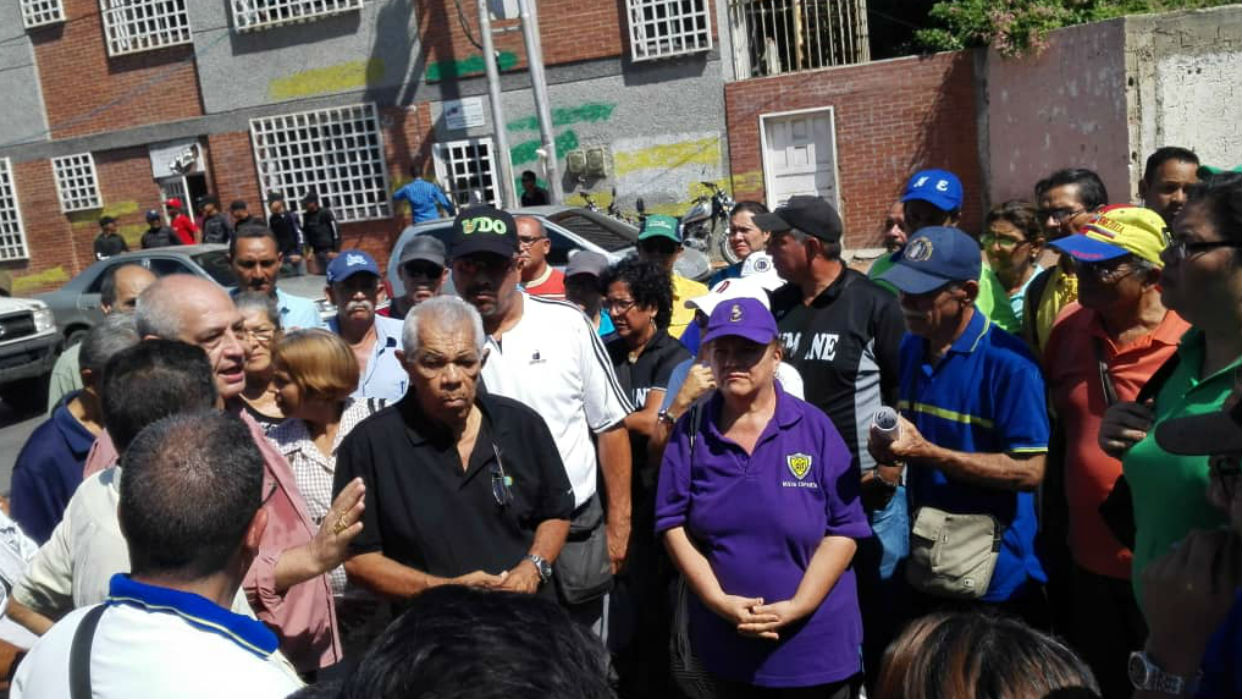
\includegraphics[width=300px]{91.jpg}%
\newline%
%
Porlamar.{-}~Miembros del Frente Amplio de Trabajadores del estado Nueva Esparta representados en 17 organizaciones gremiales y sindicales, se sumaron este viernes a la protesta nacional frente a las Inspectorías del Trabajo del país, para entregar el documento en el que ratifican la declaratoria de emergencia laboral.%
\newline%
%
A diferencia de otras instancias públicas, en la Inspectoría no hubo autoridad que recibiera el escrito, lo cual fue condenado por los trabajadores porque se supone que este es el órgano  más legítimo de defensa de sus intereses.%
\newline%
%
Ante la respuesta, acordaron dar un voto de censura al Director regional de ese despacho, Víctor Tovar.%
\newline%
%
El documento es el acuerdo alcanzado en la pasada asamblea de gremios y sindicatos que exige el reintegro de los derechos laborales de los trabajadores, méritos y beneficios logrados tras luchas reivindicativas.%
\newline%
%
Los voceros calificaron como falta de ética la posición del Inspector del Trabajo, pues aun siendo oficialistas, los diputados del Consejo Legislativo, recibieron una Comisión y escucharon sus planteamientos, en cambio la Inspectoría que debe velar por los derechos laborales negó cualquier posibilidad de diálogo.%
\newline%
%
La próxima entrega esta prevista hacerla ante la delegación regional de la Defensoría del Pueblo.%
\newline%
%
\end{document}